\section{Introduction}
% \begin{figure}
%   \centering
%   \fbox{\rule[-.5cm]{0cm}{4cm} \rule[-.5cm]{4cm}{0cm}}
%   \caption{Sample figure caption.}
% \end{figure}
Online news portals such as BBC, CNN and Google News have a huge number 
of readers daily. Many of them are anonymous or logged in as guests. 
These users typically don't read many stories in a single login session.
Given the limited interactions users engage with the portals, it is often 
hard for the systems to fully understand these news readers behavior, leading
to poor recommendation performance. 
Besides, user interests 
shift rapidly due to the dynamic nature of news articles, and this also 
results in a long tail effect. 
%A detailed data distribution is depicted in \figref{fig:data_distribution}. 
All in all, anonymous news reading
poses significant challenges to recommendation systems. 

Most news recommendation systems rely on the click streams of 
users who maintain an account. This way, they conveniently formulate 
the recommendation task as a traditional recommendation task, 
and recommend articles for users based on their collaborative 
click history~\cite{wang2018dkn, zhu2019dan}. This, however, doesn't 
apply to anonymous news reading. 
Consequently, such systems often recommend very popular items,
and has little diversity. To tackle this problem, session-based recommendation 
approaches~\cite{sottocornola2018session, garg2019sequence, xu2019time} 
are proposed, aiming to capture user intentions in short sessions. 
A \textit{session} is a sequence of user actions logged by the system
within a short time window (e.g., 30 minutes) while the user is logged on. 
Most of the approaches in this line today 
only use clicks as positive feedback of the users, which means
a user click indicates that the user likes that item. They largely ignore
all the other user actions which may be inferred from the clickstreams. 
While they may have somewhat improved the recommendation diversity,
they still suffer from the well-known cold-start problem due to
scarce user information (user cold-start) and short life span of 
news articles (article cold-start). 

% Although recommendation systems have been addressed by researchers for years, from content-based recommendation, collaborative filtering (CF), matrix factorization (MF)~\cite{rendle_factorization_2012} to delicate neural network based approaches~\cite{xin_cfm_2019}, news domain still poses some challenges compared with other items such as movies, music and books.
% \begin{itemize}
%     \item User profile could be extreme sparse. The majority of news website browsing is temporary or guest-login, and under this scenario each anonymous user is in a short session and actually read only a few stories (see \figref{fig:data_distribution}(a)). The limitation of information makes it hard to understand user's behavior.
%     \item The number of items increase dynamically. News articles are continuously generated and meanwhile their information value decays in different scale over time (see \figref{fig:data_distribution}(b)(c)). For example, news about COVID-19 pandemic may continuously attract attentions, while the name of Elon MUSK's son will soon pass into silence.
%     \item User's interests shift fast, especially when breaking news arises, such as earthquake. Besides, user's preferences are usually accompanied with randomness, making it harder to capture the information behind interactions.
% \end{itemize}

% Cold-start problem emerges when new users or new articles are introduced into the recommendation system, where users or articles are not seen during the training. While CF and MF methods have difficulty in dealing with this, many hybrid recommendation approaches thus combine content-based method to overcome cold-start problem. 

\begin{figure}[th]
    \centering
    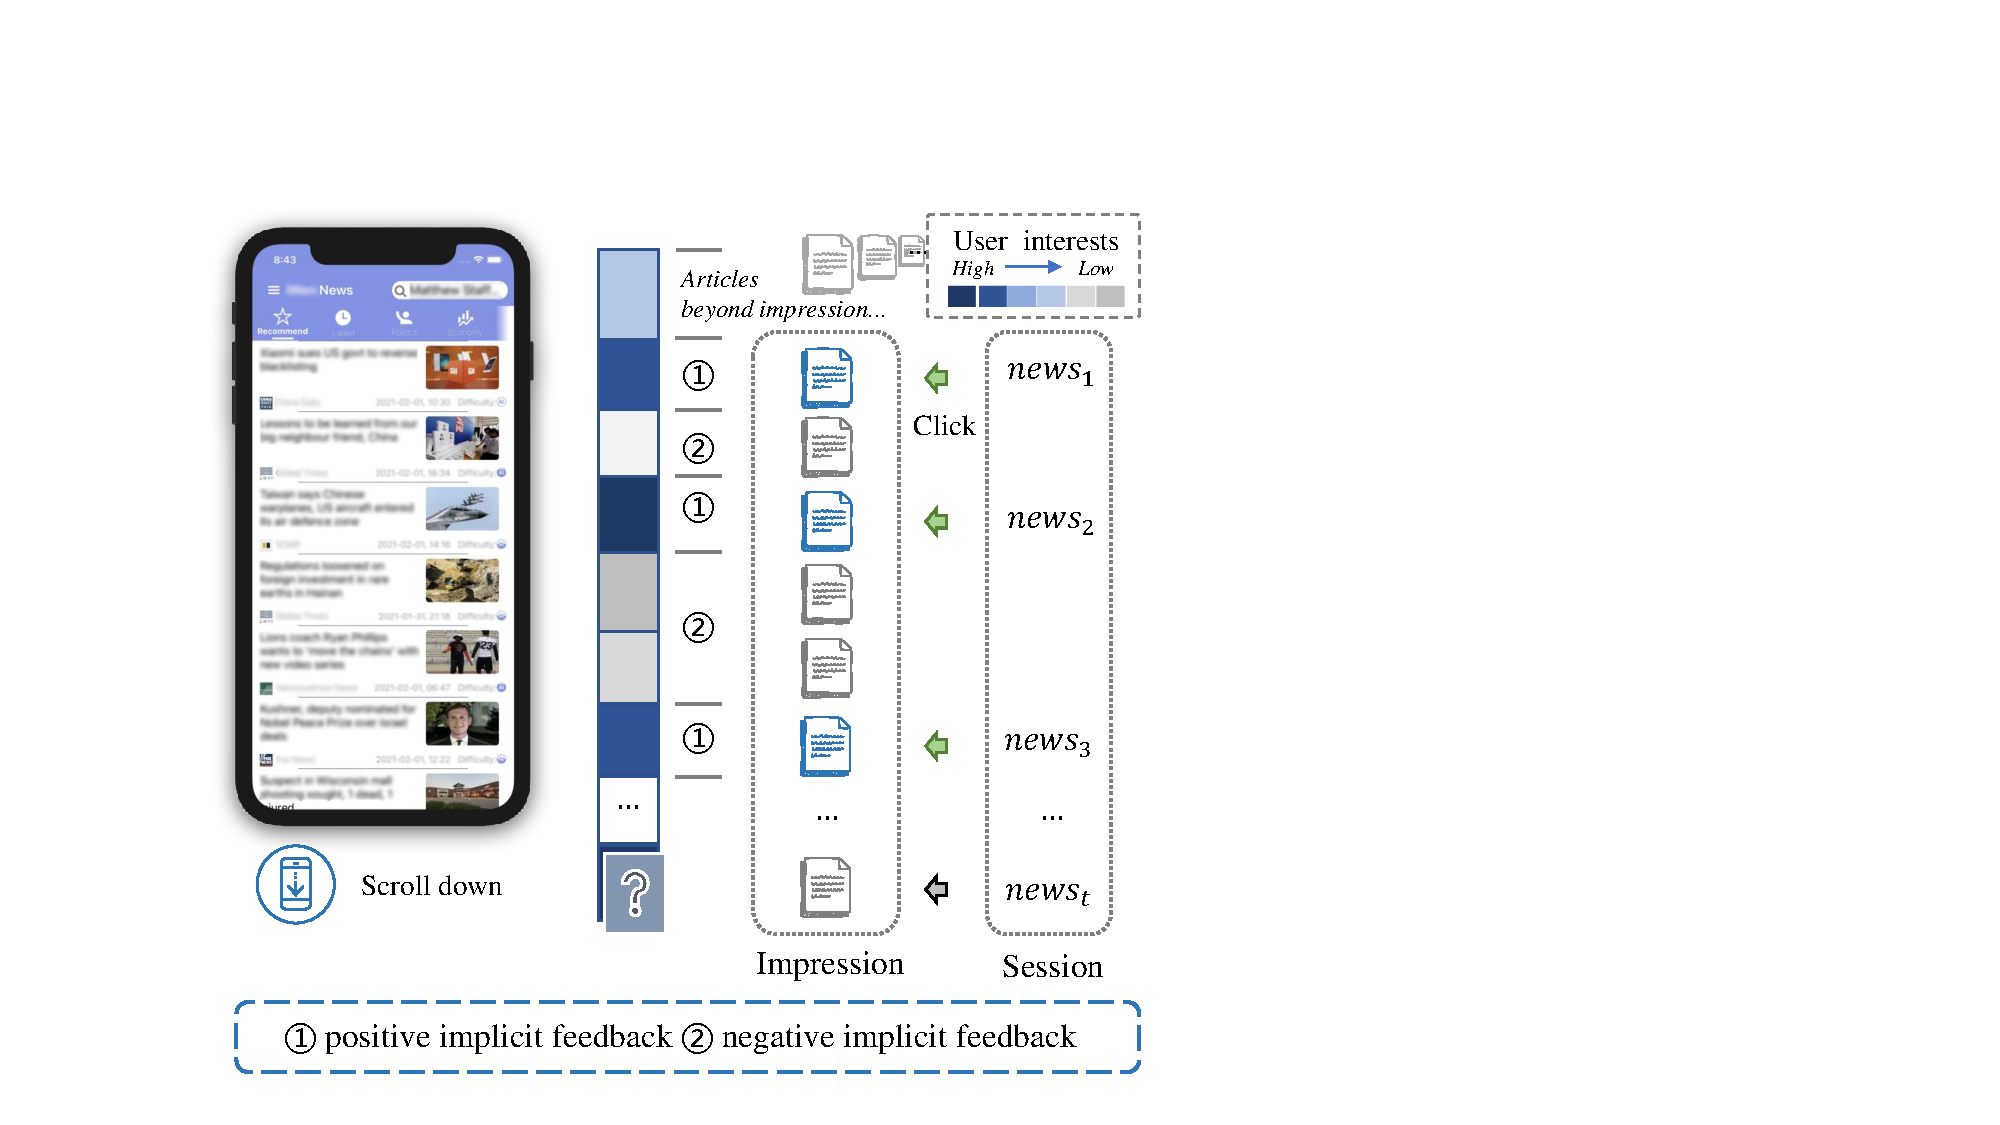
\includegraphics[width=\columnwidth]{fig/example.pdf}
    \caption{A schematic of session-based news reading by one user. 
%$news_i$ is the news articles consumed by anonymous user in a session. 
%We aim to capture users' interests through modeling their implicit feedback within a session and to predict the next-item.
}
    \label{fig:session}
\end{figure}


In this paper, we are particularly interested in exploiting user actions
other than the clicks themselves. We call them ``implicit feedback'', as
illustrated in \figref{fig:session}. 
Typical implicit feedback includes browsing the main page, 
reading an article, closing an article, etc. We believe modeling
these implicit feedback ``explicitly'' in the recommendation systems
can tackle not only diversification but also cold-start problems.
  
To infer user implicit feedback, in this paper, we focus on answering 
these two questions:
\begin{enumerate}[label=(\roman*)]
\item When a user clicks an article, does he/she really like it? 
\item If a user hasn't clicked an article, does it mean that he/she doesn't 
like it?
\end{enumerate}
The answer to both of these questions is positive for traditional click-based
recommendation systems, which provide the positive and negative feedback. While this may be true for recommending other 
commodities which are consumed offline, news consumption is a bit 
different. The reasons are listed as follows.

First, news is consumed online and in real time, and the time a user spends
on reading an article is a better, finer-grained gauge of the user's 
preference on the article, than just the click alone, which is only
binary. We model this as the implicit positive feedback in this paper.

Second, if the user didn't click on an article, it doesn't mean
he or she doesn't like it. The article may be never presented to the user.
Our view is that it's a strong negative signal if there is 
an \textit{impression} but not a click. Given that most user logs do not 
contain impression details, we want to \textit{infer} user impressions.
Our assumption is that news articles are presented to the user roughly
in the order of the time they are created or published. 
This is particularly true for anonymous users since without much user information,
the portals cannot present the news streams any other way. Our design of implicit
negative feedback will be based on this assumption in this paper. 
\figref{fig:session} shows that a user may have varying interests and thus
spend different amounts of time on different articles.

%As we know, the user usually browse news streamingly on phone's or PC's screen, the abundant news articles and limited screen size determine that a user can only be exposed to a small range impression of articles. Clearly, articles that appears in the user impression but not been viewed contains more negative meaning than articles with no interactions between them. We can leverage on this implicit negative feedback for better user intentions modeling. On the other hand, although the user clicks some articles in a session, different attention may be paid towards these articles, for example, the duration that the user stays for articles reflects user preferences. Thus, instead of regarding clicked articles as explicit positive signal, we need to model their implicit positive feedback with different weights. \figref{fig:representation} shows the two kinds of feedback: the negative implicit feedback (i.e., unclick behaviors within session impression) and positive implicit feedback (i.e., click behaviors with different attention). Compared with rich but noisy information from articles with no interactions, negative implicit feedback reflects less interests while positive implicit feedback reflects more interests. When representing user interests, rich content and temporal information can also help with exploit refined implicit feedback. 

Thus, in this paper, we formulate a session-based recommendation task 
(\secref{sec:task}) and predict the next article 
for each new session from a candidate articles pool. We design a novel 
Implicit feedback based Time \& Content Aware Recommender (ITCAR) to leverage the 
implicit feedback. Specifically, we first encode a session with the awareness 
of sequence information, articles content and positive implicit feedback, 
then we represent temporal information with content attention, 
trying to model user's reading habits (\secref{sec:positive feedback}). 
At last, we sample negative articles to jointly learn hidden vectors of user 
interests (\secref{sec:negative feedback}). 
In our experiments, we conduct offline evaluations on three datasets as 
well as different scenarios to measure the ability of ITCAR to model user 
implicit feedback (\secref{sec:experiment}).

This paper makes the following contributions: 
\begin{itemize}
    \item To the best of our knowledge, we are the first to leverage 
the positive/negative implicit feedback in anonymous session-based news recommendation;
    \item By using implicit user feedback, our model better
tackles the user cold-start problem than all other previous approches, that is, we can
make accurate prediction about annonymous users earlier in the session (see 
\secref{sec:usercold});
    \item Additionally, by proper represention of the content and  temporal information in 
the sessions, our approach better handles the article cold-start problem
(see \secref{sec:itemcold});
    \item Our comprehensive experiments on three real-world 
datasets show that ITCAR is on average 20\% more accurate than
previous SOTA methods, and better trades off the dilemma between 
diversity and accuracy (see \secref{sec:mainres}). 
\end{itemize}

The technology developed here is not only applicable for news recommendation, but also
to other streaming applications such as tweets recommendation~\cite{kwak_what_2010} 
and blogging platforms.  In some cases, recommendation systems may have access to 
user's long-term history by tracing user's identification via log-ins or cookies. 
Even in these cases, methods to excavate user's implicit feedback and 
capture the shifting of short-term interests in real-time are still valuable.
